\section{Learning NFH}

In this section, we introduce learning algorithms for the fragments $\nfhf$ and $\nfhe$. Our algorithms are based on Angluin's $\lstar$ algorithm \cite{Angluin87} for regular languages.

We first survey the $\lstar$ algorithm, and then describe the relevant adjustments for learning $\nfhe$ and $\nfhf$.

\subsubsection{The $\lstar$ algorithm}

$\lstar$ consists of two entities: a {\em learner}, who wishes to learn a DFA $A$ for an unknown (regular) language $\cal L$, and a {\em teacher}, who knows $\cal L$.
During the learning process, the learner asks the teacher two types of queries: {\em membership queries} (``is the word $w$ in $\cal L$?'') and {\em equivalence queries} (``Is $A$ a DFA for $\cal L$?'').

The learner maintains $A$ in the form of an {\em observation table} $T$ of truth values, whose rows $D, D\cdot\Sigma$ and columns $E$ are sets of words over $\Sigma$, where $D$ is prefix-closed, and $E$ is suffix-closed. Initially, $D = E = {\epsilon}$. 
For a row $d$ and a column $e$, the entry for $T(d,e)$ is $\true$ iff $d\cdot e \in{\cal L}$. The entries are filled via membership queries.
The vector of truth values for row $d$ is denoted $\row(d)$. Intuitively, the rows in $D$ determine the states of $A$, and the rows in $D\times\Sigma$ determine the transitions of $A$: the state $\row(d\cdot\sigma)$ is reached from $\row(d)$ upon reading $\sigma$. 

The learner updates the table until it is both {\em closed} and {\em consistent}. The table is closed if for every $d\in D$ and $\sigma\in \Sigma$, there is $d'\in D$ such that $\row(d') = \row(d\cdot\sigma)$. Intuitively, a closed table assures a full transition relation.
The table is consistent if for every $d_1,d_2\in D$ and every $\sigma \in \Sigma$, it holds that if $\row(d_1) = \row(d_2)$, then $\row(d_1\cdot\sigma) = \row(d_2\cdot\sigma)$. Intuitively, a consistent table assures a deterministic transition relation. 

If the table is not closed, then the missing row $d'$ is added to $D$, and $d'\cdot\sigma$ is added to $D\times\Sigma$ for every $\sigma\in \Sigma$. The new entries in $T$ are filled via membership queries. Note that this leaves $D$ prefix-closed.
If the table is inconsistent, then there is $e\in E$ for which $d_1\cdot\sigma\cdot e \neq d_2\cdot\sigma\cdot e$. The word $\sigma\cdot e$ then separates $\row(d_1)$ from $\row(d_2)$, and is added to $E$ (notice that this leaves $E$ suffix-closed). The new table entries are filled accordingly, and now $\row(d_1)\neq \row(d_2)$. 

When $T$ is closed and consistent, the learner constructs $A$: The states are the rows of $D$, the initial state is $\row(\epsilon)$, the accepting states are these in which $T(d,\epsilon) = \true$, and the transition relation is as described above. The learner then submits an equivalence query to the teacher. The teacher either confirms the equivalence, in which case the algorithm terminates, or returns a counterexample $w\in \lang{A}$ but $w\notin {\cal L}$ (which we call a {\em positive counterexample}), or $w\notin \lang{A}$ but $w\in {\cal L}$ (which we call a {\em negative counterexample}). The learner then adds $w$ and all its suffixes to $E$, and proceeds to construct the next candidate DFA $A$. 

In is shown in \cite{Angluin87} that as long as $A$ is not a DFA for the target language $\cal L$, it has less states than a minimal DFA for $\cal L$. Further, every change in the table adds at least one state to $A$. Therefore, the procedure is guaranteed to terminate successfully with a minimal DFA $A$ for $\cal L$. 

The correctness of the $\lstar$ algorithm follows from the fact that regular languages have a {\em canonical form}, which guarantees a single minimal DFA for a regular language $L$. To enable an $\lstar$-based algorithm for  $\nfhf$ and $\nfhe$, we first define canonical forms for these fragments. 


\subsection{Canonical Forms for $\nfhf$ and $\nfhe$}

Throughout this section, we discuss NFH over an alphabet $\Sigma$ with a set of variables $X = \{x_1,x_2,\ldots x_k\}$.

\subsubsection{A canonical form for $\nfhf$}

We begin with a canonical form for $\nfhf$.

Let $\A$ be an $\nfhf$. 
We say that an $\nfhf$ $\A'$ is {\em sequence complete} if for every word $w$, it holds that $\hat \A'$ accepts $w$ iff it accepts every sequence of $w$. 

\begin{lemma}
Let $\A'$ be a sequence complete $\nfhf$ over $\Sigma$ and $X$, such that 
$\hat\A'$ accepts $w$ iff $\hat\A$ accepts every sequence of $w$. 
Then $\lang{\A} =\lang{\A'}$.
\end{lemma}
\begin{proof}
For the first direction, since $\lang{\hat\A'}\subseteq \lang{\hat\A}$, we have $\lang{\A'}\subseteq \lang{\A}$.
For the second direction, let 
$S\in\lang{A}$. Then for every $v:S\rightarrow X$, it holds that $\zip(v)\in\lang{\hat\A}$. Also,   $\zip(v')\in\lang{\hat\A}$ for every sequence $v'$ of $v$. Then $\zip(v)$ and all its sequences are in $\lang{\hat\A'}$. Since this holds for every $v:X\rightarrow S$, we have that $S\in\lang{A'}$.
\end{proof}


\begin{lemma}
Every $\nfhf$ $\A$ has an equivalent sequence-complete $\nfhf$ $\A'$ over the same set of variables. 
\end{lemma}
\begin{proof}
To construct $\A'$ given $\A$, we use a similar construction to the one presented in the proof of Theorem~\ref{thm:nfhef.nonemptiness}. Essentially, for every sequence $\zeta$ of $(1,2,\ldots k)$, we construct an NFA $A_\zeta$, in which every run on a word $w$ matches a run of $\hat\A$ on $w_\zeta$. 
The $\nfhf$ $\A'$ is then obtained from $\A$ by replacing the underlying NFA with $\bigcap_{\zeta\in\Gamma} A_\zeta$, where $\Gamma$ is the set of sequences of $(1,2,\ldots k)$.
\end{proof}

\begin{lemma}
Let $\A_1$ and $\A_2$ be two sequence-complete $\nfhf$ over the same set of variables $X$.
Then $\lang{\A_1}=\lang{\A_2}$ iff  $\lang{\hat\A_1} = \lang{\hat \A_2}$.
\end{lemma}
\begin{proof}
For the first direction, let $w\in\lang{\hat\A_1}$.
Since $\A_1$ is sequence-complete, then $w'\in\lang{\hat\A_1}$ for every sequence $w'$ of $w$. Then, by the semantics of the $\forall$ quantifier, we have that $\unzip(w)\in\lang{\A_1}$ Therefore, $\unzip(w)\in\lang{\A_2}$, and so $w$ (and all its sequences) are in $\lang{\hat\A_2}$. A similar argument can be made to show that for every $w\in\lang{\hat{\A_2}}$, it holds that $w\in\lang{\hat\A_1}$. Therefore, $\lang{\hat\A_1} = \lang{\hat \A_2}$.
The second direction is trivial.
\end{proof}

Every NFA has an equivalent DFA, and DFAs have a canonical form, which is a minimal DFA. We use this property to define a canonical form for $\nfhf$ as minimal deterministic sequence-complete $\nfhf$ with a minimal number of variables. 


\subsubsection{A canonical form for $\nfhe$}

We say that an $\nfhf$ $\A'$ is {\em permutation complete} if for every word $w$, it holds that $\hat \A'$ accepts $w$ iff it accepts every permutation of $w$. 

\begin{lemma}
Let $\A$ be an $\nfhe$.
Let $\A'$ be a permutation-complete $\nfhe$ over $\Sigma$ and $X$ with the following property: for every word $w$, the underlying NFA $\hat\A$ accepts a word $w$ iff $\hat\A'$ accepts all permutations of $w$. %Notice that this is the dual property of the one listed for $\nfhf$.
Then $\lang{\A} =\lang{\A'}$.
\end{lemma}
\begin{proof}
For the first direction, since $\lang{\hat\A}\subseteq \lang{\hat\A'}$, we have $\lang{\A}\subseteq \lang{\A'}$.
For the second direction, let 
$S\in\lang{A'}$. Then there exists $v:S\rightarrow X$ such that $\zip(v)\in\lang{\hat\A'}$. Then
$\zip(v)$ is a permutation of some word $\zip(v')\in\lang{\hat\A}$.  
According to the semantics of the $\exists$ quantifier, we have that $\A$ accepts $S$. 
\end{proof}

\begin{lemma}
Every $\nfhe$ has an equivalent permutation-complete $\nfhe$ over the same set of variables. 
\end{lemma}
\begin{proof}
Similarly to the case of $\nfhf$, we construct $\A'$ given $\A$ by constructing $A_\zeta$ for every permutation $\zeta$ of $(1,2,\ldots k)$.
In this case, the $\nfhe$ $\A'$ is then obtained from $\A$ by replacing the underlying NFA with $\bigcup_{\zeta\in\Gamma} A_\zeta$, where $\Gamma$ is the set of permutations of $(1,2,\ldots k)$.
\end{proof}

\begin{lemma}
Let $\A_1$ and $\A_2$ be two permutation-complete $\nfhe$ over the same set of variables $X$.
Then $\lang{\A_1}=\lang{\A_2}$ iff  $\lang{\hat\A_1} = \lang{\hat \A_2}$.
\end{lemma}
\begin{proof}
For the first direction, let $w\in\lang{\hat\A_1}$. Then $\unzip{w}\in\lang{\A_1}$. 
Then, by the semantics of the $\exists$ quantifier, there exists some permutation $w'$ of $w$ such that $w'\in\lang{\hat\A_2}$.
Since $\A_2$ is permutation-complete, we have that $w\in\lang{\hat\A_2}$. A similar argument can be made to show that for every $w\in\lang{\hat{\A_2}}$, it holds that $w\in\lang{\hat\A_1}$. Therefore, $\lang{\hat\A_1} = \lang{\hat \A_2}$.
The second direction is trivial.
\end{proof}

We define a canonical form for $\nfhe$ as a minimal deterministic permutation-complete $\nfhe$ with a minimal number of variables.




\stam{

\subsubsection{A canonical form for $\nfhef$}

The canonical form for $\nfhef$ is a combination of the canonical forms for $\nfhf$ and $\nfhe$.

We denote an $\nfhef$ $\A$ with a quantification condition $\alpha = \exists x_1\ldots \exists x_t\forall k_{t+1}\ldots \forall x_k$ as a $(k,t)-\nfhef$. 

We say that a $(k,t)-\nfhef$ $\A$ is {\em permutation-sequence complete} if $\A$ accepts a word $w$ iff $\A$ accepts every sequence $w'$ of $w$ in which $(w'[1],\ldots w'[t])$ is a permutation of $(w[1],\ldots w[t])$. 

\begin{lemma}\label{lem:nfhef1}
Let $\A$ be a $(k,t)-\nfhef$. 
Let $\A'$ be a $(k-t)-\nfhef$, with the following property.
$w'\in\lang{\A'}$ iff $w'$ is a sequence of a word $w\in\lang{\hat\A}$ such that
\begin{enumerate}
\item
$(w'[1],\ldots w'[t])$ is a permutation of $(w[1],\ldots w[t])$. 
\item
$w_\zeta\in\lang{\hat\A}$ for every sequence $\zeta$ such that $\zeta = (1,2,\ldots t,i_{t+1},\ldots i_k)$. That is, $\hat\A$ accepts all sequences of $w$ that agree with $w$ on its first $t$ words. 
\end{enumerate}
Then $\lang{\A} = \lang{A'}$.
 \end{lemma}
\begin{proof}
For the first direction, let $S\in\lang{A}$. According to the semantics of the quantifiers, there exist $w_1,\ldots w_t\in S$, such that for every $w_{t+1},\ldots w_{k}$, it holds that $\hat\A$ accepts $\zip(w_1,\ldots w_k)$.
Then, by the semantics of the $\forall$ quantifier, $\hat\A$ accepts all words of the form $\zip(w_1,w_2,\ldots w_t,w'_{t+1},\ldots w'_k)$, where $w'_{t+1},\ldots w'_k$ are taken from $\{w_1,\ldots w_k\}$. Then, by the conditions described above, we have that $\hat\A'$ accepts $\zip(w_1,\ldots w_k)$, and therefore $S\in\lang{A'}$.

For the second direction, let $S\in\lang{A'}$. 
Then there exist $w_1,\ldots w_t\in S$, such that for every $w_{t+1},\ldots w_{k}$, it holds that $\hat\A'$ accepts $w' = \zip(w_1,\ldots w_k)$.
Then, by the conditions described above, $w'$ is a sequence of a word $w\in\lang{A}$ such that $\{w[1],\ldots w[t]\} = \{w'[1], \ldots w'[t]\} = \{w_1,\ldots w_t\}$ (though these words do not necessarily appear in the same order in $w,w'$), and such that $w[i] = w'[i]$ for every $t<i\leq k$. 
Then, by the semantics of the quantifiers, we have that $S\in\lang{\A}$.
\end{proof}

Notice that the $\nfhef$ $\A'$ of Lemma~\ref{lem:nfhef1} is permutation-sequence complete.

\begin{lemma}
Every $(k,t)-\nfhef$ $\A$ has an equivalent permutation-sequence complete $(k,t)-\nfhef$ $\A'$.
\end{lemma}
\begin{proof}
We construct $\A'$ in two steps. 
First, we construct $\A''$ that is the intersection of every $\A_\zeta$ for a sequence $\zeta$ of the form $(1,2,\ldots t, i_{t+1},\ldots i_k)$, as for $\nfhf$ over the last $k-t$ indices, and then we construct $\A'$ as the union of $\A''_\xi$ for every permutation $\xi$ of the form $(i_1,\ldots i_t,t+1,\ldots k)$, as for $\nfhe$ over the first $t$ indices.
\end{proof}

\begin{lemma}
Let $\A_1$ and $\A_2$ be two permutation-sequence complete $(k,t)-\nfhef$.
Then $\lang{\A_1}=\lang{\A_2}$ iff  $\lang{\hat\A_1} = \lang{\hat \A_2}$.
\end{lemma}
\begin{proof}
Suppose that $\lang{\A_1}=\lang{\A_2}$. Let $w\in\lang{\hat\A_1}$. 
Since $\A_1$ is permutation-sequence complete, we have that $w_\zeta\in\lang{\A_1}$ for every sequence $\zeta$ of the form $(1,\ldots t,i_{t+1},\ldots i_k)$. By the semantics of the quantifiers, we have that $\unzip{w}\in\lang{A_1}$.
Therefore, $\unzip{w}\in\lang{A_2}$, and so, according to the semantics of the quantifiers and the order of words in $w$, 
there exists a word $w'\in\lang{\hat\A_2}$ such that $(w'[1],\ldots w'[t])$ is a permutation of $(w[1],\ldots w[t])$, and $(w'[t+1],\ldots w'[k])$ is a permutation of $(w[t+1],\ldots w[k])$. Since $\A_2$ is permutation-sequence complete, we have that $w\in\lang{\hat\A_2}$. A similar argument shows that $\lang{\hat\A_2}\subseteq \lang{\hat\A_1}$.
The second direction is trivial.
\end{proof}

\begin{lemma}
Let $\A$ be a $(k,t)-\nfhef$, such that $k$ is the minimal number of variables needed for expressing $\lang{\A}$.
Then $\hat\A$ accepts a word $w$ in which $w[1],\ldots w[t]$ are all distinct. 
\end{lemma}
\begin{proof}
Suppose by way of contradiction that for every $w\in\lang{\hat\A}$, two of the first $t$ words of in $w$ are equal. Due to the semantics of the $\exists$ quantifier, we can also 
\end{proof}


\begin{lemma}
Let $\A_1$ and $\A_2$ be permutation-sequence complete $\nfhef$ for the same hyperlanguage $\cal L$, both with a minimal set of variables. Then the quantification conditions of $\A_1$ and $\A_2$ are equal.
\end{lemma}
\begin{proof}
Suppose that $\A_1$ is a $(t,k)-\nfhef$, and $\A_2$ is a $(t,m)-\nfhef$.
Suppose by way of contradiction, and without loss of generality, that $t < m$. 
Let $S\in\lang{\A_1}$. 
\end{proof}

We define a canonical form for $\nfhef$ as a minimal deterministic permutation-sequence complete $\nfhef$ with a minimal number of variables. 


}% of stam












\subsection{Learning $\nfhf$ and $\nfhe$}

We now describe learning algorithms for $\nfhe$ and $\nfhf$, based on the $\lstar$ framework.
These algorithms aim to learn minimal deterministic sequence-complete (in the case of $\nfhf$) or permutation-complete (in the case of $\nfhe$) NFH, with a minimal number of variables, for a target hyperlanguage $\hl$.

In the case of hyperautomata, the membership queries and the counterexamples provided by the teacher consist of hyperwords. We assume that the teacher returns a minimal counterexample in terms of size of the hyperword. 

During the procedure, the learner maintains an NFH $\A$ via the current number of variables $k$ and an observation table for $\hat\A$, over the alphabet $\hat\Sigma  = (\Sigma\cup\{\#\})^k$, where $k$ is initially set to $1$. 
When the number of variables is increased to $k'>k$, the alphabet of $\hat\A$ is extended accordingly to $(\Sigma\cup\{\#\})^{k'}$. 
To this end, we define a function $\uparrow_k^{k'}:(\Sigma\cup\{\#\})^k\rightarrow (\Sigma\cup\{\#\})^{k'}$, which replaces every word $(\sigma_1,\ldots \sigma_k)$, with $(\sigma_1,\ldots \sigma_k,\ldots \sigma_k)$. That is, the last letter is duplicated to create a $k'$-tuple. 
We extend $\uparrow_k^{k'}$ to words: $\uparrow_k^{k'}(w)$ is obtained by replacing every letter $\sigma$ in $w$ with $\uparrow_k^{k'}(\sigma)$. 
Notice that if $\unzip(d\cdot e) \in \lang{\A}$, then $\unzip(\uparrow_k^{k'}(d\cdot e)) \in \lang{\A}$. 
Therefore, when the number of variables is increased, every word $w$ in the rows and columns of $T$ is replaced with $\uparrow_k^{k'}(w)$. 


\subsubsection{Learning $\nfhf$}

In the case of $\nfhf$, when the teacher returns a counterexample $S$, it holds that if $|S|> k$, then the counterexample must be positive. Indeed, assume by way of contradiction that the teacher returns a negative counterexample $S$. Then for every $k$ words $w_1,w_2,\ldots w_k$ in $S$, it holds that $zip(w_1,w_2,\ldots w_k)\in \lang{\hat\A}$, but $S\notin \hl$. Therefore, in an $\nfhf$ $\A'$ for $\hl$, there exists some word of the form $w = \zip(w_1,w_2,\ldots w_k)$ such that $w_i\in S$ for $1\leq i \leq k$, and $w\notin \lang{\hat\A'}$. As a result, $\{w_1,w_2,\ldots w_k\}\notin \hl$. Since $\zip(w_1,w_2,\ldots w_k)$ and all its sequences are in $\lang{\hat\A}$, then a smaller counterexample is $\{w_1,w_2,\ldots w_k\}$, a contradiction to the minimality of the counterexample $S$. 

In fact, if $|S|>k$ then it must be that $|S| = k+1$. Indeed, since $S$ is a positive counterexample, and $\A$ accepts all representations of subsets of size $k$ of $S$ (otherwise the teacher would return counterexample of size $k$), then there exists a subset $S'\subseteq S$ of size $k+1$ that should be represented, but is not. Therefore, $S'$ is a counterexample of size $k+1$.

As a conclusion, when a counterexample $S$ of size $k+1$ is returned, the learner updates $k\leftarrow k+1$, updates $T$ by updating every $w\in D\cup D\cdot {\hat\Sigma} \cup E$ to $\uparrow_k^{k+1}(w)$, arbitrarily selects a permutation $p$ of the words in $S$, and adds  $\zip(S)$ and all its suffixes to $E$.
In addition, it updates $D\cdot\hat\Sigma$ in accordance with the new updated $\hat\Sigma$, and fills in the missing entries accordingly.  

When $|S| \leq k$, then the counterexample is either positive or negative.
If $S$ is positive, then there exists some permutation $p$ of the words in $S$ such that $\A$ does not accept $\zip(p)$. (a permutation and not a proper sequence, otherwise there would be a smaller counterexample). The learner finds such a permutation $p$, and adds $\zip(p)$ and all its suffixes to $T$. Notice that $\zip(p)$ does not already appear in $T$, since a membership query would have returned ``yes'', and so $\A$ would have accepted $\zip(p)$.

if $S$ is negative, then $\A$ accepts all sequences of length $k$ of words in $S$, though it should not.
Then there exists a permutation $p$ of the words in $S$ that does not appear in $T$, and which $\A$ accepts. The learner then finds such a permutation $p$ and adds $\zip(p)$ and all its suffixes to $T$.

It holds, that if $p$ is a permutation of the words in $S$, and $S$ is a negative counterexample, then $\zip(p)$ should not be in $\lang{\hat\A}$ due to any other hyperword $S$, and if $S$ is a positive counterexample, then it should be in $\lang{\hat\A}$ for every $S'$ such that $S\subseteq S'$. Therefore, the above actions by the learner are valid.  

When an equivalence query succeeds, then $\A$ is indeed an $\nfhf$ for $\hl$. However, it may be the case that $\A$ is not sequence-complete, as $\hat\A$ may accept a word $w = \zip(w_1,\ldots w_k)$ but not all of its sequences. This check can be performed by the learner directly on $\hat\A$. 
Notice that $w$ does not occur in $T$, since a membership query on $w$ would return ``no''. 
Once it is verified that $\A$ is not sequence-complete, the counterexample $w$ (and all its suffixes) are added to $T$, and the procedure returns to the learning loop.
 
As we have explained above, variables are added only when necessary, and so the output $\A$ is indeed an NFH for $\hl$ with minimally many variables. 
The correctness of $\lstar$ and the minimality of the counterexamples returned by the teacher guarantee that for each $k'\leq k$, the run learns a minimal deterministic $\hat\A$ for hyperwords in $\hl$ that are represented by $k'$ variables. Therefore, a smaller $\hat\A'$ for $\hl$ does not exist, as restricting $\hat\A'$ to the first $k'$ letters in each $k$-tuple would produce a smaller underlying automaton for $k'$ variables, a contradiction. 

\begin{figure}[ht]
%\hrulefill
    \begin{center}
        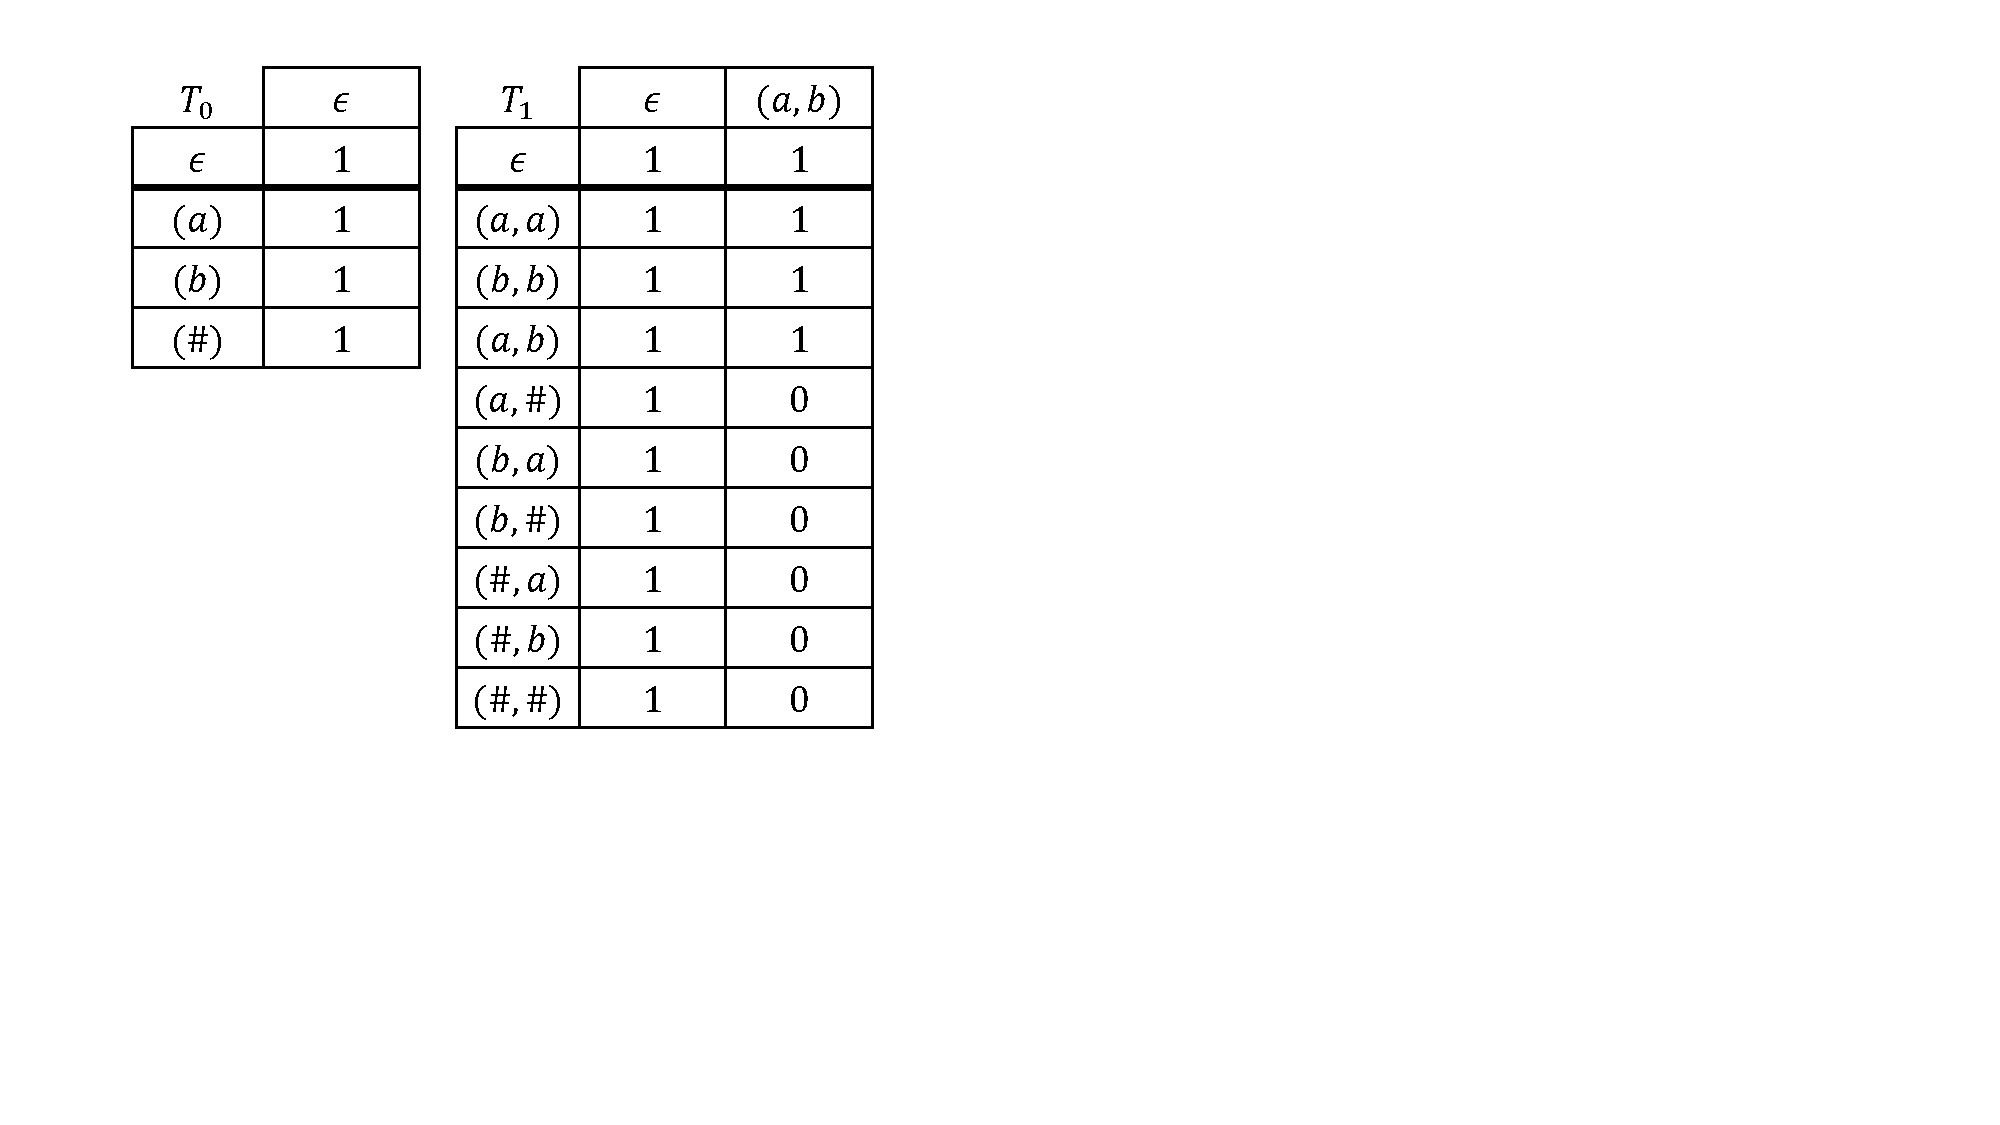
\includegraphics[scale=0.5]{figures/learning_nfhf.pdf}
    \end{center}
    \caption{The first stages of learning $\lang{\A_3}$ of Figure~\ref{fig:nfh_examples}.}
    \label{fig:learning_nfhf}
%    \hrulefill
\end{figure}

\begin{example}
Figure~\ref{fig:learning_nfhf} displays the first two stages of learning $\hlang{\A_3}$ of Figure~\ref{fig:nfh_examples}.
$T_0$ displays the initial table, with $D=E = \{\epsilon\}$, and $\hat\Sigma = \{a,b,\#\}$. since $\{a\}, \{b\}$, and $\{\epsilon\}$ are all in $\hlang{\A_3}$, the initial NFH $\A$ that the learner constructs is over a single variable, and includes, according to the answers from the membership queries, a single accepting state.

Since $\hlang{\A_3}$ includes all hyperwords of size $1$, which are now accepted by $\A$, the smallest positive counterexample the teacher can return is a hyperword of size $2$, which, in the example, is $\{a,b\}$. Table $T_1$ is then obtained from $T_0$ by applying $\uparrow_1^2$, updating the alphabet $\hat\Sigma$ to $\{a,b,\#\}^2$, and updating $D\cdot\hat\Sigma$ accordingly. The table is filled by submitting membership queries. For example, for $(b,a)\in D\cdot\hat\Sigma$ and $(a,b)\in E$, the learner submits a membership query for $\{ba, ab\}$, for which the teacher returns ``no''.
\end{example}

\subsubsection{Learning $\nfhe$}

The learning process for $\nfhe$ is almost similar to the one for $\nfhf$. We briefly describe the differences. 


As in $\nfhf$, relying on the minimality of the counterexamples returned by the teacher guarantees that when a counterexample $S$ such that $|S|>k$ is returned, it is a positive counterexample. 
Indeed, assume by way of contradiction that $S$ is a negative counterexample of size $k'$. Since $\hat\A$ accepts $S$, there exists a word $\zip(w_1,\ldots w_k)$ in $\lang{\hat\A}$ such that $\{w_1,\ldots w_k\}\in S$. According to the semantics of $\exists$, if $\zip(w_1,w_2,\ldots w_k)$ in $\lang{\hat\A}$ then $S\in\hlang\A$. Since $S\notin\hl$, we have that $\{w_1,\ldots w_k\}$ is a smaller counterexample, a contradiction. 

Therefore, when the teacher returns a counterexample $S$ of size $k'>k$, the alphabet $\hat\Sigma$ is extended to $(\Sigma\cup\{\#\})^{k'}$, and the table $T$ is updated by $\uparrow_{k}^{k'}$, as is done for $\nfhf$.

If $|S|\leq k$, then $S$ may be either positive or negative. If $S$ is negative, then there exists some permutation $w$ of $S$ that is accepted by $\hat\A$. However, no such permutation is in $T$, as a membership query would have returned ``no''. Similarly, if $S$ is positive, then there exists no permutation of $S$ that $\hat\A$ accepts. In both cases, the learner chooses a permutation of $S$ and adds it, along with its suffixes, to $E$. 

As in the case of $\nfhf$, the success of an equivalence query does not necessarily imply that $\A$ is permutation-complete. 
If $\A$ is not permutation-complete, the learner finds two words $w,w'$ such that $w\in\lang{\hat\A}$ but $w'\notin\lang{\hat\A}$, and adds $w'$ as a counterexample to $E$. It holds that $w'$ was not in $T$ prior to this addition.
The procedure then returns to the learning loop.

